\section{Discussion \& Limitations}

\textbf{Regression-based motion mapping}
There are two different approaches to achieving inverse rig mapping: one is optimization based approach that is similar to our method, and the other is a regression-model-based approach that requires example data.
The benefit of the regression based approach lies in performance because the required runtime computation is simple interpolation of the example data. Thus, this approach can be a good alternative with a sufficient number of high quality examples. 
However, creating the example data is not an easy task. The artist is required to create \textit{good} example motion data per each character rig. The \textit{good} is also hard to define, because the examples should cover the entire range of motion. If the artist provides example data with different rig parameters for a single pose, it may cause conflict in a regression model.
Although real-time performance is an appealing benefit, it is not an essential requirement in the inverse motion mapping because it is one-time process in the production pipeline.
As a future work, it would be a good idea to use a regression model for an unbiased automatic uniform sampling for the entire skeletal configuration that is constrained by the range of motion.

\textbf{Keyframe reduction}
Our optimization results in a dense key frame data because we optimize each pose of character motion.
The dense keyframes are not convenient to edit for an artist, so we perform a keyframe reduction\cite{seol2011artist} for each rig parameter after the motion mapping process. Key pose extraction from motion data is another alternative\cite{halit2011multiscale}.
Both of the methods are applicable in the production pipeline. 

\textbf{Limitations}
If the character rig has full body rig controllers such as full body IK, our rig analysis process cannot group the parameters, because the entire skeletal segments are connected to every rig space parameter.
However, the main purpose of the rig analysis is to increase the efficiency in optimization by dividing the problem into a set of sub-problems.
Therefore, although the full body rig controller can decrease the performance, the mapping can be done without any problem.
Our method successfully maps the motion to rigs even in these cases.

Our optimization is based on the Jacobians of rig and skeletal parameters.
If the skeletal parameter remains unchanged in a specific range of the rig space parameters, our solution can overgrow in the range.
For example, the fully stretched IK end effector controllers(Figure~\ref{fig:limit}, left) and the translational IK pole vector controllers(Figure~\ref{fig:limit}, right) have infinite solutions occurred the specific ranges as indicated by the blue line and the blue plane in Figure~\ref{fig:limit}.
The infinite solution occrued by the use of IK controllers is well known, and it can be simply solved by clamping\cite{buss2004introduction} after the motion mapping. Providing an automatic parameter clamping when parameters have infinite solutions in a specific range can be a direction for future work.

\begin{figure}[!ht]
\centering
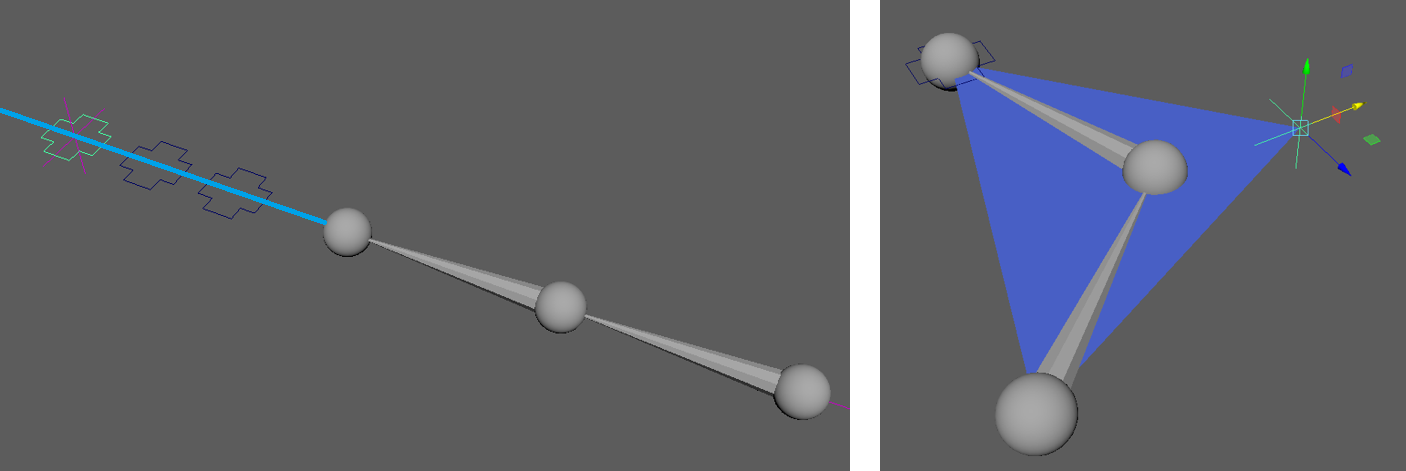
\includegraphics[width=3.0in]{images/ikProblem}
\caption{(left) Fully stretched IK end effector problem (right) IK pole vector controller problem}
\label{fig:limit}
\end{figure}
